
\documentclass[twoside,twocolumn]{article}

% ------
% Fonts and typesetting settings
\usepackage[sc]{mathpazo}
\usepackage[T1]{fontenc}
\linespread{1.05} % Palatino needs more space between lines
\usepackage{microtype}
\usepackage{amsmath}
\usepackage{tikz}
\tikzstyle{na} = [baseline=-.5ex]
\usetikzlibrary{shapes,graphs,graphs.standard,quotes,shapes.geometric,arrows,fit,calc,positioning,automata,chains,snakes,decorations.pathreplacing}
\newcommand{\tikzmark}[2]{\tikz[remember picture,baseline=(#1.base)]{\node[inner sep=2pt] (#1) {#2};}}
\tikzset{
    instrtext/.style = {font=\fontsize{25}{22.4}\selectfont},
    instrbit/.style = {font=\fontsize{20}{22.4}\selectfont}
}

\setlength{\belowcaptionskip}{-5pt}

% ------
% Page layout
\usepackage[hmarginratio=1:1,top=32mm,bottom=40mm,columnsep=20pt]{geometry}
\usepackage[font=it]{caption}
\usepackage{paralist}
%\usepackage{multicol}

\usepackage{graphicx}


% ------
% Lettrines
\usepackage{lettrine}

% ------
% Abstract
\usepackage{abstract}
	\renewcommand{\abstractnamefont}{\normalfont\bfseries}
	\renewcommand{\abstracttextfont}{\normalfont\small\itshape}


% ------
% Titling (section/subsection)
\usepackage{titlesec}
\renewcommand\thesection{\Roman{section}}
\titleformat{\section}[block]{\large\scshape\centering}{\thesection.}{1em}{}


% ------
% Header/footer
%\usepackage{fancyhdr}
%	\pagestyle{fancy}
%	\fancyhead{}
%	\fancyfoot{}
%	\fancyhead[C]{}
%	\fancyfoot[RO,LE]{\thepage}


\usepackage{color}

% ------
% Maketitle metadata
\title{\vspace{-7mm}%
	\fontsize{24pt}{10pt}\selectfont
	\textbf{CCOPI: Implementing a custom coprocessor interface for
    VexRiscv}
	}	
\author{%
	\large
	\textsc{Jens Nazarenus, Dominik Swierzy} \\[2mm]
	\normalsize	RheinMain University of Applied Sciences \\
    \normalsize	jens.nazarenus@hs-rm.de, dominik.swierzy@hs-rm.de
	%\vspace{-5mm}
	}
\date{\today}

\usepackage[utf8]{inputenc}

\usepackage{hyperref}


%%%%%%%%%%%%%%%%%%%%%%%%
\begin{document}

\maketitle
%\thispagestyle{fancy}

\begin{abstract}
\noindent In this paper we introduce CCOPI, a custom coprocessor interface for the
RISC-V implementation VexRiscv. CCOPI as well as VexRiscv is written in
the hardware description language SpinalHDL. The interface is responsible 
for the communication between the coprocessor and the core CPU pipeline of 
VexRiscv and thus helps hardware developers in the designing process of 
a coprocessor with a custom instruction-set extension.

CCOPI uses the fexibility of the RISC-V implementation VexRiscv to create 
the interface. This paper also shows how VexRiscv is designed particulary with 
regard to modifications and custom extensions. 
\end{abstract}

\section{Introduction}
Coprocessors in general are used to support the core CPU(s) with the
calculation of specific mathematical operations. A coprocessor aims to
accelerate this specific task over a software implementation of the same
task.

Former coprocessors like the Intel 80387 or Motorolas 68881 were used to
execute IEEE 754 compliant floating point operations and could be
bought as independent components. To use the coprocessors new
instructions were included in the instruction stream of the core CPU.

Today the logic of coprocessors are often included inside the CPU
itself as an instruction set extension. Well-known examples are the
Intel\textregistered{} x87 
floating point unit (FPU) or the Intel\textregistered{} Advanced Encryption Standard New 
Instructions (AES-NI). Both modules introduce new instructions which can
be used by developers.
CCOPI is designed to produce coprocessors which resides inside the core
RISC-V CPU named VexRiscv similar to x87 or AES-NI discussed above.

Before approaching the main topic CCOPI and its implementation, this paper
gives an introductional overview of the topics RISC-V and the used
hardware description language SpinalHDL.
\section{RISC-V}
RISC-V is the name of an open source instruction set architecture (ISA)
which has been developed at the University of California, Berkeley.
The ISA describes the instructions any RISC-V implementation must
implement, plus optional extensions. The required minimum is specifed in
the ``Base Integer Instruction Set'' of the User Level ISA.

A RISC-V instruction $instr$ is always decoded in 32 bits.

       \begin{figure}[h]
        \centering
        \resizebox{7.25cm}{!}{
            \begin{tikzpicture}[]
                %% R-type
                \draw[] (0,6) -- (31,6);
                \draw[] (0,7) -- (31, 7);
                \draw[] (0,6) -- (0,7);
                \draw[] (31,6) -- (31,7);

                \draw[] (31-7,6) --(31-7,7);
                \draw[] (31-12,6) --(31-12,7);
                \draw[] (31-15,6) --(31-15,7);
                \draw[] (31-20,6) --(31-20,7);
                \draw[] (31-25,6) --(31-25,7);

                \node[instrtext] at (31-25-3,6.5) {funct7};
                \node[instrtext] at (31-19-3.5,6.5) {rs2};
                \node[instrtext] at (31-15-2.5,6.5) {rs1};
                \node[instrtext] at (31-12-1.5,6.5) {funct3};
                \node[instrtext] at (31-7-2.5,6.5) {rd};
                \node[instrtext] at (31-0-3.5,6.5) {opcode};

                %% bit header
                \node[instrbit] at (0+0.3,7+0.5) {31};
                \node[instrbit] at (31-7-0.3, 7+0.5) {7};
                \node[instrbit] at (31-12-0.5, 7+0.5) {12};
                \node[instrbit] at (31-12+0.5, 7+0.5) {11};
                \node[instrbit] at (31-15-0.5, 7+0.5) {15};
                \node[instrbit] at (31-15+0.5, 7+0.5) {14};
                \node[instrbit] at (31-20+0.5, 7+0.5) {20};
                \node[instrbit] at (31-20-0.5, 7+0.5) {19};
                \node[instrbit] at (31-25+0.5, 7+0.5) {24};
                \node[instrbit] at (31-25-0.5, 7+0.5) {25};
                \node[instrbit] at (31-7+0.3, 7+0.5) {6};
                \node[instrbit] at (31-0.3, 7+0.5) {0};

                %%\node[instrtext] at (33, 6.4) {R-Type};

            \end{tikzpicture}
        }

        \caption[Instruktionstypen]{R-Type}      
        \label{fig:riscv_r_type}
    \end{figure}
\noindent The notation $instr[fromBit:toBit]$ is used to extract information from
the instruction. In figure \ref*{fig:riscv_r_type} $instr[6:0]$
represents the opcode of the instruction, which is used ...
\section{SpinalHDL}
\section{VexRiscv Overview}
\subsection{Pipeline}
\subsection{Plugin mechanism}
\section{CCOPI}
\section{Acceleration Evaluation}

\bibliographystyle{unsrt}
\bibliography{literature}

\end{document}
